\documentclass{salt}

% This document template was developed by the editors of /Semantics and
% Pragmatics/ and minimally modified to work with the salt.cls document class.

%\usepackage[equation]{gb4e-salt}
%\noautomath

\usepackage{tcolorbox}
\usepackage{natbib}
\usepackage{linguex}

% macros for example annotations
\def\bad{{\leavevmode\llap{*}}}
\def\marginal{{\leavevmode\llap{?}}}
\def\verymarginal{{\leavevmode\llap{??}}}
\def\swmarginal{{\leavevmode\llap{4}}}
\def\infelic{{\leavevmode\llap{\#}}}



%\interfootnotelinepenalty=10000

%=====================================================================
%========================= preamble material =========================

% Metadata for the PDF output. ASCII-only!
\pdfauthor{Swantje Toennis and Judith Tonhauser}
\pdftitle{German clefts address unexpected questions}
\pdfkeywords{German clefts, QUD, discourse expectations}

% Short title inside square brackets, for the running headers.
% If no short title is given, no title appears in the headers.
% Please use sentence case for the title.
\title[German clefts address unexpected questions]{German clefts address unexpected questions%
  \thanks{We thank the SALT32 reviewers and audience, the ELM2 reviewers and audience, as well as audiences at Potsdam University and the University of Stuttgart for valuable feedback and fruitful discussions.}
}

% Optional short author inside square brackets, for the running headers.
% If no short author is given, no authors print in the headers.
\author[Swantje T\"onnis, Judith Tonhauser]{%
  % As many authors as you like, each separated by \AND.
  \saltauthor{Swantje T\"onnis \\ \institute{University of Stuttgart}} \AND
  \saltauthor{Judith Tonhauser \\ \institute{University of Stuttgart}} %\AND
  %\saltauthor{Author3 \\ \institute{Institute3}}%
}

%=====================================================================

\begin{document}

%=====================================================================
%============================ frontmatter ============================

\maketitle

% First page headers and page numbers; update these when you are assigned final
% page numbers
%
% the page number of the first page of this paper
\setcounter{page}{1}

% Create the first page headings.
% This needs to be issued *after* \maketitle.
% \firstpageheadings{<volume>}{<first page>}{<last page>}{<year>}{}{}
\firstpageheadings{32}{000}{000}{2022}{}{}

\begin{abstract}  
In this paper, we provide empirical evidence for \citeauthor{tonnis_2021}' (\citeyear{tonnis_2021}) hypothesis that German cleft sentences address relatively unexpected questions in discourse while their canonical variants address relatively expected questions. We present an experiment that measures the relative preference between the German cleft and its canonical variant in contexts that differ with respect to how expected the question is that they answer. The expectedness of the question was measured separately in a norming study. The result of the experiment supports analyses of German clefts that take discourse expectations into account when analyzing the acceptability of clefts in contrast to canonical sentences. Approaches that primarily focus on differences in exhaustivity \cite[e.g.,][]{deveaugh-geiss_et_al_2018b} or contrast \cite[e.g.,][]{rochemont_1986} need to be adapted in order to account for the results.
\end{abstract}

\begin{keywords}
  German clefts, discourse expectations, question expectedness, questions in discourse
\end{keywords}

%=====================================================================
%============================ article text ===========================


%============================ introduction ===========================
\section{Introduction}
\label{sec:intro}
The German \textit{es}-cleft, exemplified in \ref{cleft}, is a rather infrequent construction in German, compared to clefts in languages like French. Contexts in which the cleft is preferred over its canonical variant, exemplified in \ref{canonical}, are rare. The context in \ref{context3} represents such a case \cite[inspired by][]{tonnis_2021}: The cleft is preferred over the canonical sentence in \ref{context3}. In many other contexts, e.g., in \ref{context1}, the preference is reversed.

\ex. Als Benni in den Schuppen kam, war sein Fahrrad zugestellt.\\\textit{`When Benni came into the shed his bicycle was blocked.'}\label{context1} 

 \ex. Als Benni in den Schuppen kam, war sein Fahrrad zugestellt. Er konnte es so schnell nicht frei bekommen. Also fuhr er mit dem Tretroller los. \\\textit{`When Benni came into the shed his bicycle was blocked. He couldn't get it out quickly enough. So he set off on the scooter.'}\label{context3} 
 \a.\label{canonical} Lilly hat vor Bennis Fahrrad geparkt.\hfill \checkmark\hspace{0.1em} in \ref{context1}, ? in \ref{context3}\\
\textit{`Lilly parked in front of Benni's bicycle.'}
\b.\label{cleft}Es war Lilly, die vor Bennis Fahrrad geparkt hat.\hfill? in \ref{context1}, \checkmark\hspace{0.1em} in \ref{context3}\\
\textit{`It was Lilly who parked in front of Benni's bicycle.'}

\cite{tonnis_2021} argued that previous approaches to clefts which primarily focused on exhaustivity, uniqueness, or contrastivity cannot account for this contrast \cite[e.g.,][]{prince_1978,horn_1981,rochemont_1986,velleman_et_al_2012}. Instead, \cite{tonnis_2021} hypothesized that the acceptability of German clefts is sensitive to the expectedness of the question addressed: while clefts address questions that are relatively unexpected in discourse, their canonical variants address relatively expected questions. The question addressed by \ref{canonical} and \ref{cleft} in both contexts above is \textit{Who parked in front of Benni's bicycle?}. Following \cite{tonnis_2021}, we argue that this question is relatively more expected in context \ref{context1} than in context \ref{context3} because the story has moved on to a different topic in the latter context. Consequently, the cleft is more acceptable in contexts such as \ref{context3}, and the canonical variant in contexts such as \ref{context1}, as predicted by \cite{tonnis_2021}.

In this paper, we provide empirical evidence for \citeauthor{tonnis_2021}' (\citeyear{tonnis_2021}) hypothesis. We developed a novel experiment paradigm designed to measure question expectedness (norming study). In the main experiment, we investigated the hypothesis by collecting relative preference ratings for the cleft and its canonical variant in contexts which differ with respect to how expected the question addressed by the two variants~is.

The paper is structured as follows: In \autoref{subsec:prev_analyses}, we summarize prior approaches to clefts, and show that they cannot capture the contrast in \ref{context1} and \ref{context3}. In \autoref{subsec:expect}, the analysis developed in \cite{tonnis_2021} is presented. In \autoref{sec:exp}, we present the experiment. In \autoref{sec:discussion}, we discuss theoretical and methodological implications of our results and specific details of our stimuli. \hyperref[sec:conclusions]{Section~\ref*{sec:conclusions}} concludes.


%============================ background ===========================
\section{The discourse-sensitivity of clefts}
\label{sec:background}

%============================ previous analyses ===========================

\subsection{Previous approaches to clefts}
\label{subsec:prev_analyses}

On some prior approaches, a cleft contributes an inference that is either weaker or not present for its canonical variant. On \citeauthor{percus_1997}' (\citeyear{percus_1997})  analysis, for instance, clefts trigger a uniqueness presupposition that is not triggered by their canonical variants. The presupposition is contributed by a definite description from which the cleft is derived: The cleft in \ref{percus1} triggers the presupposition that there is a unique individual that parked in front of Benni's bicycle, derived from the definite description in \ref{percus2}. 

\ex.\a.\label{percus1} It was Lilly who parked in front of Benni's bicycle.
	\b.\label{percus2} The one who parked in front of Benni's bicycle was Lilly.
	
This analysis cannot account for the contrast in \ref{context1} and \ref{context3} because the two contexts do not differ with respect to the relevant presupposition; specifically, neither context satisfies the presupposition. Consequently, \citeauthor{percus_1997}' (\citeyear{percus_1997})  analysis predicts that the cleft is either unacceptable in both contexts (because the presupposition is not satisfied) or acceptable in both (if the presupposition can be accommodated). Either way, \cite{percus_1997} does not predict the contrast observed in \ref{context1} and \ref{context3}.

Other analyses considered the cleft to have an exhaustivity inference \cite[e.g.,][]{buring_kriz_2013,horn_1981}. The cleft in \ref{percus1} has the exhaustivity inference in \ref{exh}.
\ex.\label{exh} Nobody other than Lilly parked in front of Benni's bicycle.

\cite{deveaugh-geiss_et_al_2018b} found in a picture-verification-task that the exhaustivity inference of German clefts was stronger than for canonical sentences. \cite{deveaugh-geiss_et_al_2015} found that the German cleft was judged as less acceptable than the canonical sentence when followed by an exhaustivity violation, as indicated in the English translation in \ref{exh_violated}. 
\ex.\label{exh_violated} 
\a.?\label{exh_violated-a}It was Lilly who parked in front of Benni's bicycle, and Anna as well.
\b.\label{exh_violated-b}Lilly parked in front of Benni's bicycle, and Anna as well.

By contrast, the corpus study by \cite{pavlovic_2019} suggested that German clefts do not necessarily contribute an exhaustivity inference, as there were many occurrences of clefts with additive particles in the pivot (i.e., \textit{It was also Lilly who...}). Similarly, we observe that the cleft in \ref{context3}, repeated in \ref{exh_context3}, does not appear to contribute exhaustivity: The cleft with the exhaustivity violation in \ref{cleft_exh} is acceptable and is still preferred over the canonical variant \ref{canonical_exh}. This data suggests that analyses on which clefts mainly differ from their canonical variants by an exhaustivity inference cannot account for the contrast in \ref{context1} and \ref{context3}.
\ex. \textit{When Benni came into the shed his bicycle was blocked. He couldn't get it out quickly enough. So he set off on the scooter.}\label{exh_context3} 
 \a.?\label{canonical_exh}Lilly hat vor Bennis Fahrrad geparkt und Anna auch.\\
\textit{`Lilly parked in front of Benni's bicycle, and Anna as well.'}
\b.\label{cleft_exh}Es war Lilly, die vor Bennis Fahrrad geparkt hat, und Anna auch.\\
\textit{`It was Lilly who parked in front of Benni's bicycle, and Anna as well.'}

Another line of prior research was concerned with contrastivity in clefts. \cite{rochemont_1986}, for instance, argued that clefts express contrastive focus while their canonical variants are compatible with both information and contrastive focus. This approach does not capture the contrast in \ref{context1} and \ref{context3}, either, because the two contexts do not differ with respect to contrastivity according to the criteria for contrast in \cite{repp_2010}. Specifically, the two contexts do not differ in terms of the set of (explicit) alternatives to Benni (no additional individuals are mentioned in either context). Hence, the contrast in contexts \ref{context3} and \ref{context1} cannot be explained by arguing that the conditions for a contrastive statement differ in the two contexts.


% Discourse-related approaches to clefts
Other previous approaches analyzed the cleft in its wider discourse context, and investigated how the cleft, compared to its canonical variant, is integrated into the previously constructed discourse structure.  Corpus studies on English clefts \cite[a.o.,][]{prince_1978,hedberg_1990}, for instance, showed that it is not always possible to replace a natural occurrence of a cleft in its context with its canonical variant without loosing text coherence. Consider the pair of examples from \citet[471]{delin_oberlander_1995} in \ref{d&o}: the naturally occurring discourse with the cleft in \ref{d&o_cleft} is coherent. In contrast, the variant in \ref{d&o_canonical}, in which the cleft is replaced by its canonical variant, is incoherent. 

\ex.\label{d&o}\a.\label{d&o_cleft} Doubling the selling space to 700 square feet was not to be the greatest expense. \textbf{It was the new fixtures and fittings to fill this space that would be costly.}
\b.?\label{d&o_canonical}Doubling the selling space to 700 square feet was not to be the greatest expense. \textbf{The new fixtures and fittings to fill this space would be costly.}

We take this data as evidence that the discourse structure needs to be considered to fully capture the acceptability of the cleft in comparison to its canonical variant.
\cite{velleman_et_al_2012} presented such an analysis, which is based on questions in discourse. They treated clefts as inquiry-terminating constructions, as in example \ref{pizza1} \citep[a slightly adapted version of][449]{velleman_et_al_2012}. 

\ex.\label{pizza1}A: What did Mary eat?\\
B: I thought she said she was gonna get a pasta dish, but I might be wrong.\\
A: And did she also order a salad?\\
C: Guys, I was there and actually paid attention. \textbf{It was a pizza that
Mary ate.}

\citet[][]{velleman_et_al_2012} claimed that speaker C uses the cleft to mark the ongoing inquiry with respect to the question \textit{What did Mary eat?}~as terminated. This analysis does not capture the contrast in \ref{context1} and \ref{context3}, either. First, the cleft in \ref{cleft} does not even contribute to the ongoing inquiry, which would be about what Benni did or about where Benni went. The question which is actually addressed by the cleft in \ref{context3} (\textit{Who parked in front of Benni's bicycle?}), is not one which is being discussed, it is rather a question which had been ignored and is now picked up again. Second, the inquiry about this question might be terminated by uttering the cleft, but not necessarily. The author could also continue discussing this question, e.g., as in \ref{cleft_exh}. 
 
Finally, \cite{destruel_velleman_2014} proposed an analysis which involves the discourse structure as well as contrastivity. They argued that the acceptability of the cleft is affected by violations of expectations on the content level \ref{destruel_velleman_contrast-a} as well as on the discourse level \ref{destruel_velleman_contrast-b}.

\ex.\label{destruel_velleman_contrast} \textit{Conflict with expectations}: Clefts are more felicitous the more they conflict with interlocutors' expressed expectations.
\a.\label{destruel_velleman_contrast-a} \textit{Expectations about the world}: These expectations may involve beliefs about the world, expressed as assertions or presuppositions. More strongly expressed beliefs lead to stronger conflict.
\b.\label{destruel_velleman_contrast-b} \textit{Expectations about the discourse}: These expectations may involve beliefs about the direction in which the discourse is going, expressed, among other ways, by marking content as at-issue or not-at-issue.\\
\textcolor{white}{}\hfill\cite[199]{destruel_velleman_2014}

In their study, \cite{destruel_velleman_2014} investigated clefts in the corrective function. They manipulated the discourse context with respect to whether the antecedent of the correction was provided as at-issue or as not-at-issue content. The examples in \ref{destruel_velleman1} and \ref{destruel_velleman2} are taken from their study \cite[][212--213]{destruel_velleman_2014}. They argued that the antecedent \textit{Leah convinced him to buy it} is not-at-issue in \ref{destruel_velleman1} while it is at-issue in \ref{destruel_velleman2}. One of their main findings was that the cleft was strongly preferred over the canonical sentence when the antecedent was not-at-issue, as in \ref{destruel_velleman1}, as opposed to when it was at-issue, as in \ref{destruel_velleman2}.

\ex.I can't believe Mark bought that ugly car. It looks like it's about to fall apart, too. 
\a.\label{destruel_velleman1}I have no idea how Leah convinced him to buy it. \hfill[not-at-issue]\\
-- Actually, it was Anna who convinced him. \hfill[cleft preferred]
\b.\label{destruel_velleman2}And it turns out that Leah convinced him to buy it.\hfill[at-issue] \\
-- Actually, Anna convinced him. \hfill[canonical sentence preferred]

%Still, the contrast in \ref{context1} and \ref{context3} cannot be explained entirely. 
This difference is predicted by their hypothesis, in particular part \ref{destruel_velleman_contrast-b}: Since the antecedent of the correction is marked as not-at-issue in \ref{destruel_velleman1} the interlocutors' expectations are violated more strongly than in the case of the at-issue marked antecedent in \ref{destruel_velleman2}. Hence, the cleft is correctly predicted to be more felicitous in \ref{destruel_velleman1} than in \ref{destruel_velleman2}. 

Following the hypothesis in \ref{destruel_velleman_contrast}, the contrast in \ref{context1} and \ref{context3} can be explained: One could hypothesize that the interlocutors' expectations differ in the two contexts with respect to what the next sentence is about. The expectations that the next sentence is about who parked in front of Benni's bicycle are stronger in \ref{context1} than in \ref{context3}, because the text moved on to a new topic in \ref{context3} (Benni choosing the scooter instead of the bicycle). Hence, the cleft violates the expectations more strongly in \ref{context3} compared to \ref{context1} and is, thus, predicted to be more felicitous in \ref{context3} than in \ref{context1}. In contrast to \posscitet{destruel_velleman_2014} examples, the contexts \ref{context1} and \ref{context3} do not differ with respect to at-issueness: In both contexts, the antecedent content that somebody parked in front of Benni's bicycle is implied by the first context sentence, which is identical in the two contexts. Thus, this content is not at-issue in both contexts. Hence, the differing expectations about discourse are not signaled in \ref{context1} and \ref{context3} by explicitly marking content as either at-issue or not at-issue. Rather, as proposed in \cite{tonnis_2021}, the two contexts differ in the status of the question addressed by the cleft and the canonical sentence. This analysis is introduced next.


%============================ my analysis ===========================
\subsection{German clefts and expectations in discourse}
\label{subsec:expect}


Analyzing the discourse functions of German clefts,\footnote{The analysis is restricted to focus-background clefts, such as (i-a), where the pivot represents the focus. Topic comment clefts, as in (i-b), where the cleft pivot is the topic and the relative clause contains new information, are not covered. Main stress is marked in capital letters in the examples.
\ex.[(i)] \textit{When Benni came into the shed his bicycle was blocked. He couldn't get it out quickly enough. So he set off on the scooter.}
\a.\label{fb_cleft}It was LILLY who parked in front of Benni's bicycle.
\b.\label{tc_cleft}It was Benni who CRASHED the scooter later that day.

}
\cite{tonnis_2021} argued that most of the cases in which a German cleft is acceptable can be subsumed under one discourse function \cite[a related analysis is presented by][]{delin_oberlander_1995}. \citeauthor{tonnis_2021} hypothesized that clefts are used to address a relatively unexpected question, and canonical sentences are used to address a relatively expected question. 

One of the assumptions underlying this hypothesis is that every sentence addresses a question, which may be implicit or expressed by an interrogative sentence \cite[following][]{roberts_2012}. As in \cite{zimmermann_2011b}, \cite{tonnis_2021} proposed that interlocutors form expectations about the direction in which the discourse is going.  According to her model, each possible question that could be asked or answered in the next discourse move is paired with an expectedness value (values between 0 and 1). This value represents the likelihood that the next discourse move is going to address the respective question. In context \ref{context3}, the question \textit{Where did Benni go with the scooter?}~is assigned a rather high value (i.e., close to 1), while the question \textit{How was the weather in Colombia?}~is assigned a value close to 0. Diverging from \citeauthor{roberts_2012}' (\citeyear{roberts_2012}) model, any question may be addressed (not just the one at the top of a stack), as long as it exceeds a certain expectedness threshold. This approach is in line with \cite{kehler_rohde_2017}, who analyzed the discourse expectations as a probability distribution over questions the ensuing utterance is likely to answer.

Furthermore, \cite{tonnis_2021} argued that the distribution of expectedness values is updated after each new sentence because a sentence can affect the distribution. Sentence \ref{pq}, for instance, gives rise to the question Q \textit{Why did Mary scold John?} \citep[e.g.,][]{onea_2016}. In other words, asserting \ref{pq} would strongly raise the expectedness value of Q. This, in turn, would reduce the expectedness of other questions because all expectedness values have to sum up to 1 (like in a probability distribution).
\ex.\label{pq} Mary scolded John.

\posscitet{kehler_rohde_2017} findings on implicit causality verbs (e.g., \textit{scold}) support this observation: In implicit causality contexts, participants produced significantly more \textit{why}-questions than in non-implicit causality contexts as, for instance, in \textit{Mary saw John}.

A factor which reduces the expectedness value of a yet unanswered question is a greater distance to the sentence which raised that question. In other words, when an author decides to not address a question immediately, the reader will expect less and less that the question will still be addressed. This is also a side effect of new questions becoming more expected, since this automatically reduces the expectedness of other questions \cite[273ff.]{tonnis_2021}. For illustration, consider again the two contexts in \ref{context1} and \ref{context3}, repeated here:
\ex.[\ref{context1}] \textit{When Benni came into the shed his bicycle was blocked.}

\ex.[\ref{context3}] \textit{When Benni came into the shed his bicycle was blocked. He couldn't get it out quickly enough. So he set off on the scooter.}

The first sentence in \ref{context1} and \ref{context3} gives rise the question Q \textit{Who parked in front of Benni's bicycle?}. The word triggering Q is \textit{zugestellt} `blocked', which describes a resultative state but leaves open the source of this resultative state. This can be argued to give rise to Q, which is asking for this source. In context \ref{context3}, there are new questions arising due to the second and the third sentence, such as \textit{What else could Benni use instead of the bicycle?}~or \textit{Where did Benni go with the scooter?}. Those questions are then relatively more expected than Q, and would cause the expectedness value of Q to decrease. 

These assumptions about discourse being structured by questions, and question expectedness decreasing with intervening sentences suffice to account for the contrast between the cleft and the canonical sentence in \ref{cleft-canonical} in the contexts \ref{context1} and \ref{context3}. 

\ex.\label{cleft-canonical}
 \a.\label{canonical10} Lilly hat vor Bennis Fahrrad geparkt.\hfill \checkmark\hspace{0.1em} in \ref{context1}, ? in \ref{context3}\\
\textit{`Lilly parked in front of Benni's bicycle.'}
\b.\label{cleft10} Es war Lilly, die vor Bennis Fahrrad geparkt hat.\hfill ? in \ref{context1}, \checkmark\hspace{0.1em} in \ref{context3}\\
\textit{`It was Lilly who parked in front of Benni's bicycle.'}

Following \cite{tonnis_2021}, we hypothesize that the question Q is relatively more expected in the context in \ref{context1} than in the context in \ref{context3}. Given \citeauthor{tonnis_2021}' (\citeyear{tonnis_2021}) hypothesis that German clefts are used to address relatively unexpected questions and canonical sentences address relatively expected questions, it is predicted that the cleft in \ref{cleft10} is judged to be more acceptable in context \ref{context3} than in context \ref{context1}, and that the canonical sentence in \ref{canonical10} is judged to be more acceptable in context \ref{context1} than in context \ref{context3}.

This analysis naturally extends to the example in \ref{pizza2}, which \cite{velleman_et_al_2012} identified as problematic for their own analysis:

\ex.\label{pizza2}
\a.[A:] What did Mary eat?
\b.[B:] ?It was a pizza that Mary ate. \hfill \cite[449]{velleman_et_al_2012}

The question addressed by the cleft, namely what Mary ate, is relatively expected, given that it is contributed by the immediately preceding interrogative sentence. Therefore, the analysis developed in \cite{tonnis_2021} correctly predicts that the cleft is dispreferred here over the canonical sentence. By contrast, the same question is less expected in \ref{pizza1}, where the conversation has already moved on to a different question (\textit{Did she also order a salad?}). Consequently, the cleft is correctly predicted to be acceptable here \cite[for a more detailed discussion see][133--141]{tonnis_2022}.


%============================ experiment ===========================

\section{Experiment}
\label{sec:exp}

We ran an experiment designed to investigate \citeauthor{tonnis_2021}' (\citeyear{tonnis_2021}) hypothesis that German cleft sentences address relatively unexpected questions in discourse while their canonical variants address relatively expected questions. Participants rated the relative acceptability of a cleft and its canonical sentence variant in a context in which the question addressed by the cleft and its canonical sentence variant was more or less expected. Question expectedness was normed prior to the experiment.\footnote{\label{github}The materials of the experiment and the norming study, as well as the data and R code for generating the figures and analyses reported on in this article are available at \url{https://github.com/swantje-toennis/expectations_cleft}. The norming study and the experiment were preregistered: norming study at \url{https://osf.io/sb8d7}, main experiment at \url{https://osf.io/pd29h}. Informed consent was obtained.}



\subsection{Participants} 120 self-declared native speakers of German, recruited and paid (\pounds9.10 per hour) on \href{https://www.prolific.co/}{Prolific}, participated in the experiment (53 female, 66 male, 1 non-binary; ages 18--71 years, mean age 31).

\subsection{Materials} 
\label{subsec:material}

The target sentences were pairs of a German canonical sentence and its cleft sentence variant, as shown in \ref{pair1} and \ref{pair2}, respectively. The two members of a pair convey the same proposition (here, that Lilly parked in front of Benni's bicycle), but differ in their form. There were 16 pairs of target sentences. The full set of stimuli is provided in Supplement A in the GitHub repository mentioned in footnote \ref{github}.


\ex.\label{pair} \a.\label{pair1} Lilly hat vor Bennis Fahrrad geparkt. \\
\textit{`Lilly parked in front of Benni's bicycle.'}
\b.\label{pair2} Es war Lilly, die vor Bennis Fahrrad geparkt hat.\\
\textit{`It was Lilly who parked in front of Benni's bicycle.'}

For each of the pairs of target sentences, we created a German target context sentence that gives rise to a question that is addressed by the respective target sentence. This question is referred to as the target question. The context sentence for the pair in \ref{pair} is given in \ref{context1_rep2}: This context sentence gives rise to the target question \textit{Who parked in front of Benni's bicycle?}, which is addressed by both sentences in \ref{pair}. 

\ex.\label{context1_rep2} Als Benni in den Schuppen kam, war sein Fahrrad zugestellt. \\ \textit{`When Benni came into the shed his bicycle was blocked.'}

Each target stimulus consisted of a pair of target sentences, such as \ref{pair}, that was preceded by a context in one of two context conditions. In the first context condition, the context consisted only of the target context sentence, as in \ref{context1_rep2}. In the second context condition, the context consisted of the target context sentence as well as two additional sentences that carried the story on, as in \ref{context3_rep2}. 

\ex.\label{context3_rep2} Als Benni in den Schuppen kam, war sein Fahrrad zugestellt. Er konnte es so schnell nicht frei bekommen. Also fuhr er mit dem Tretroller los.\\ \textit{`When Benni came into the shed his bicycle was blocked. He couldn't get it out quickly enough. So he set off on the scooter.'}

The construction of each context followed the same principle. The target context sentence always consisted of two clauses: a temporal clause, which located an individual's actions in time (e.g., when Benni came into the shed), and a main clause which introduced a problematic state for the individual (such as Benni's bicycle being blocked). The target context sentences all contained a state adjective/participle, such as {\em zugestellt} `blocked'. In the condition where the context consisted of three sentences, the second context sentence further described this problematic state (such as it being impossible to free the bicycle quickly). By contrast, the third context sentence always described a new event, temporally located after the event denoted in the temporal clause of the target context sentence (such as Benni leaving on his scooter). This temporal progression was also indicated by a discourse marker, such as {\em also} `so' or {\em schließlich} `eventually'.

We assumed that the target question was relatively more expected immediately after the target context sentence, that is, when the context only consisted of the target context sentence, as in \ref{context1_rep2}, and relatively less expected when two additional sentences that carried the story on had occurred after the target context sentence, as in \ref{context3_rep2}. We therefore refer to these two context conditions as the `higher expectedness' and the `lower expectedness' conditions, respectively. Our assumption was confirmed by a norming study, in which 80 self-declared native speakers of German gave slider ratings (from 0 to 100) about how expected the target questions (as well as four other questions that varied in their expectedness) were in the two context conditions.\footnote{None of the participants of the norming study later participated in the main experiment. Details of the norming study can be found in Appendix A of this paper.} \autoref{fig:results_exp1} plots the mean expectedness ratings of the target questions by context condition. As expected, the mean expectedness ratings of the target questions were higher immediately after the target context sentence (i.e., in the higher expectedness context condition) than when the target context sentence was followed by two additional sentences (i.e., in the lower expectedness context condition).

\begin{figure}[]
\centering
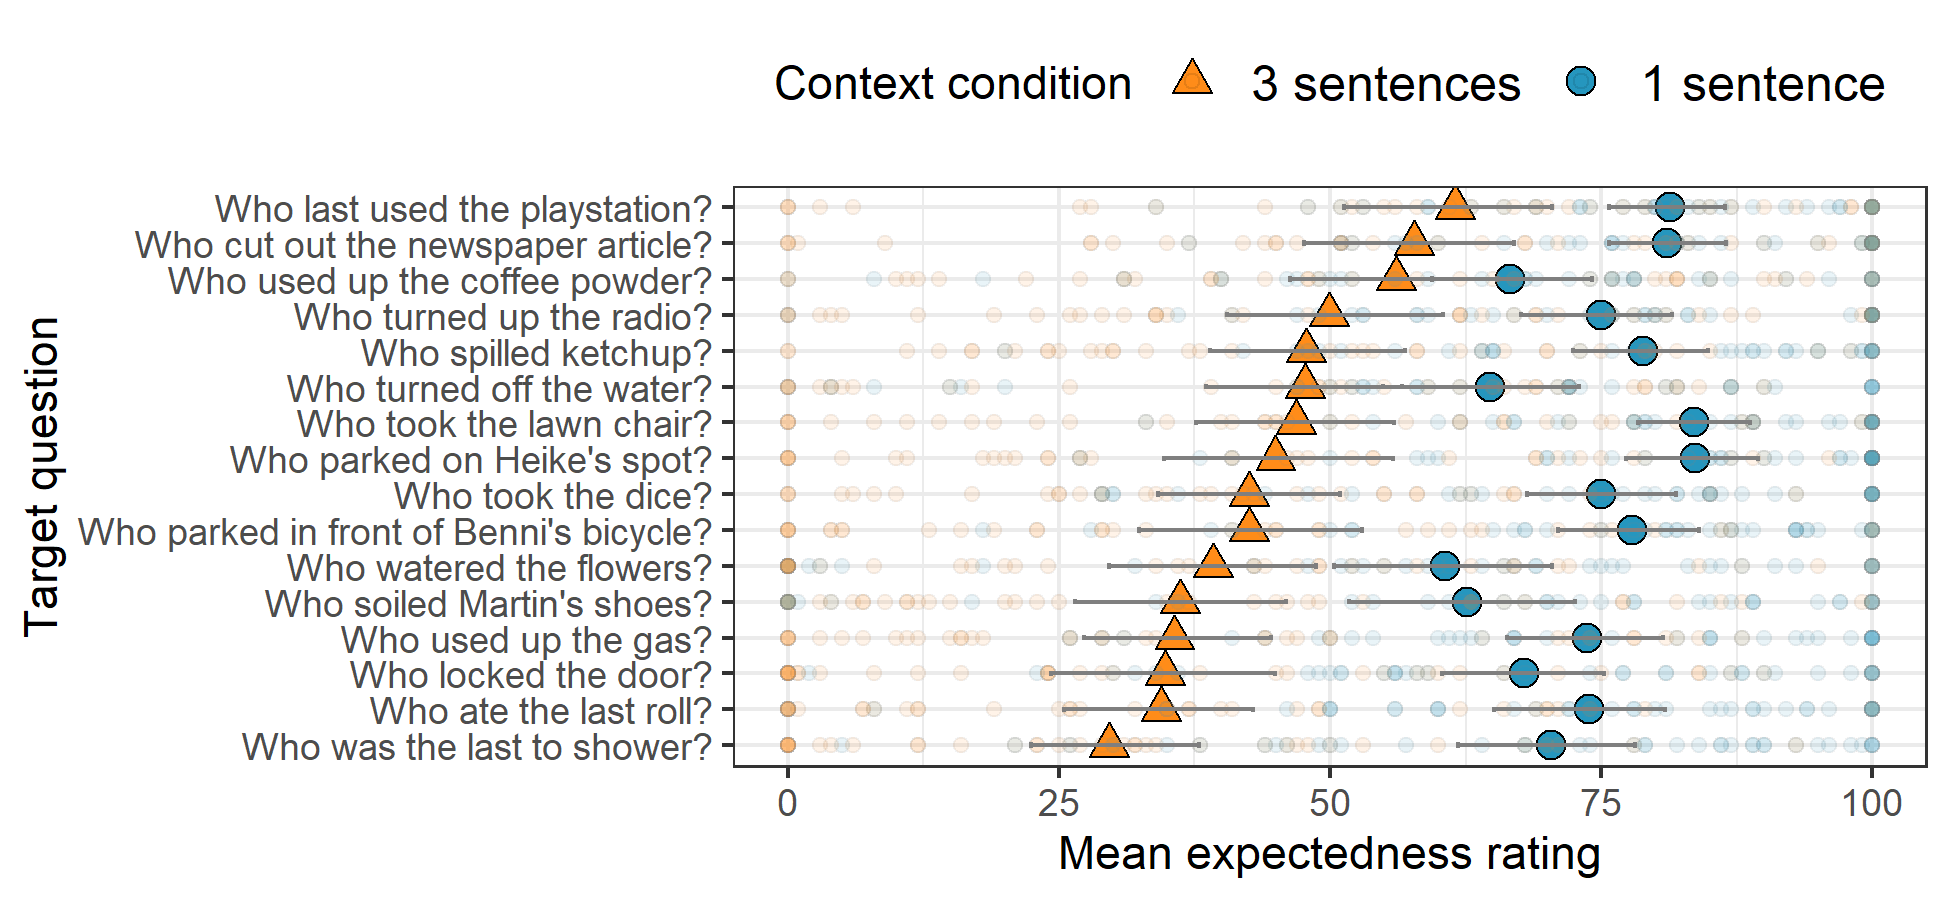
\includegraphics[width=\textwidth]{results_norming_by_question.png}
\caption{Mean expectedness of the (English translations of the) target questions by context condition in the norming
study. Error bars indicate 95\% bootstrapped confidence intervals. Transparent
dots indicate individual participants' ratings.}\label{fig:results_exp1}
\end{figure}

The 32 target stimuli were distributed across eight lists such that each list had four distinct items (where an item is a combination of a target context sentence and its corresponding pair of target sentences): two in the higher expectedness condition and two in the lower expectedness condition. Each list also included the same eight filler stimuli and the same four control stimuli, for a total of 16 stimuli per list. As clefts are very infrequent in German, we only included four target stimuli on each list, to mitigate against participants realizing that the experiment was about clefts. The filler and control stimuli both consisted of a context and a pair of sentences, like the target stimuli. The contexts of the filler stimuli consisted of one, two, or three sentences, and the pairs of sentences differed in their discourse properties, such as the presence of a discourse marker, or whether a determiner phrase was fronted or occurred in situ. 

The control stimuli consisted of two one sentence and two three sentence contexts. Each pair of sentences denoted the same proposition but differed in whether a target referent was referred to by a pronoun or a definite description, as illustrated in \ref{control_example1} and \ref{control_example2}. Two of the controls were like \ref{control_example1}: They involved a non-salient referent (the computer). This referent was introduced in the first sentence of the context and referred to after two intervening sentences. Here, we expected the definite description variant in \ref{control_example1b} to be preferred over the pronoun variant because non-salient referents are referred to by more complex referring expressions, like a definite description \cite[see][]{gundel_et_al_1993}. The computer (masculine in German) was the only suitable antecedent for the masculine pronoun \textit{er} `he'. Other later introduced entities were excluded as an antecedent because they had a different gender, here the feminine gender of \textit{Freundin} `female friend'. The other two controls, such as \ref{control_example2}, involved a very salient referent, introduced by a infinite description in the context sentence (here, a colleague from Poland that he is friends with). Here, we expected the pronoun variant in \ref{control_example2a} to be preferred over the definite description because salient antecedents are referred to by a less complex form, such as a pronoun \cite[see][]{gundel_et_al_1993}.  The full set of filler and control stimuli is given in Supplement A of the GitHub repository mentioned in footnote \ref{github}.

\ex.\label{control_example1} Heike kam in ihr Arbeitszimmer und hat den Computer hochgefahren. Dann hat sie eine Mail an eine Freundin geschrieben. Sie hat eine halbe Stunde dafür gebraucht.\\
\textit{`Heike came into her office and booted the computer$_{masc}$. Then, she wrote an email to her friend$_{\mbox{\footnotesize fem}}$. It took her half an hour.'}
\a. Er war sehr langsam.\\
\textit{`It$_{masc}$ was very slow.'}
\b.\label{control_example1b} Der Computer war sehr langsam.\\
\textit{`The computer was very slow.'}


\ex.\label{control_example2} Martin hat eine befreundete Arbeitskollegin aus Polen nach Hause eingeladen.\\
\textit{`Martin invited home a colleague$_{\mbox{\footnotesize fem}}$ from Poland that he is friends with.'}
\a.\label{control_example2a} Sie hat eine Flasche Rotwein mitgebracht.\\
\textit{`She$_{\mbox{\footnotesize fem}}$ brought a bottle of wine.'}
\b. Die befreundete Arbeitskollegin aus Polen hat eine Flasche Rotwein mitgebracht.\\
\textit{`The colleague$_{\mbox{\footnotesize fem}}$ from Poland that he is friends with brought a bottle of wine.'}

\subsection{Procedure}

At the beginning of the experiment, participants were introduced to a family of six that live together: the children Lilly and Benni, their parents Heike and Martin, and their grandparents Irmgard and Wilhelm. The participants were told that they would read short texts about events describing the family's everyday life in and around the house.

On each trial, participants were shown a text and a pair of sentences, consisting of a cleft and its canonical variant: one of the sentences was labeled `A' and the other one `B'. Participants were told that the next sentence of the text, marked by `XXXX', is illegible. Participants were instructed to rate which of the sentences, A or B, they would prefer as the continuation of the text, and to indicate the strength of their preference by adjusting a slider marked `(A viel besser)' (A much better) on the left end, `(B viel besser)' (B much better)  on the right end, and `(beide gleich gut)' (both equally good) in the middle. The order of the two members of a pair was randomized on each trial. Slider ratings were coded as a value between -100 (absolute preference of the canonical sentence over the cleft) and 100 (absolute preference of the cleft over the canonical sentence). An English translation of a sample trial in the lower expectedness condition is given in \autoref{fig:stimulus_exp2}. After completing the experiment, participants filled out a short demographic survey (age, gender, education, native language, foreign languages with level, and region where the participant grew up).

\begin{figure}[]
\caption{\small English translation of a sample trial in lower expectedness condition of the relative preference rating with A = canonical sentence and B = cleft.}
\footnotesize Read the text in the box. The next sentence of this text is illegible (marked by XXXX).
\begin{tcolorbox}
\textit{When Benni came into the shed his bicycle was blocked. He couldn't get it out quickly enough. So he set off on the scooter.} \textbf{XXXX}
\end{tcolorbox}\vspace{1ex}
A. \textbf{Lilly parked in front of Benni's bicycle.}\\
B. \textbf{It was Lilly who parked in front of Benni's bicycle.}\vspace{1ex}

Which of the sentences A or B would you prefer and how strongly? Adjust the slider accordingly.


\includegraphics[width=\textwidth]{slider.png}

(A much better)\hspace{21ex} (both equally good)\hfill (B much better)\normalsize
\label{fig:stimulus_exp2}
\end{figure}


\subsection{Data exclusion} 

The data from 27 participants was excluded from the analysis because their preference rating on at least one control stimulus deviated from the group mean by more than two standard deviation in the opposite direction of what we expected. Data from 93 participants entered the analysis (40 female, 52 male, 1 non-binary, age range 18--71 years, mean age 31).

\subsection{Results}

\autoref{fig:results_exp2} plots the mean preference rating by context condition, i.e., by the expectedness of the target question. As predicted, the mean preference rating is higher (indicating a stronger preference towards the cleft) in the lower expectedness condition than in the higher expectedness condition. This result suggests that participants' preference ratings of the cleft and its canonical variant are sensitive to how expected the target question was. Specifically, the cleft was rated as more preferred over the canonical sentence in the lower expectedness condition, that is, when the target question was relatively less expected, than in the higher expectedness condition, that is, when the target question was relatively more expected.

\begin{figure}[]
\caption{Mean preference rating with 95\% bootstrapped confidence intervals by context condition. Kernel probability density of the individual participants' mean ratings, given in transparent dots, overlaid.}
\begin{center}
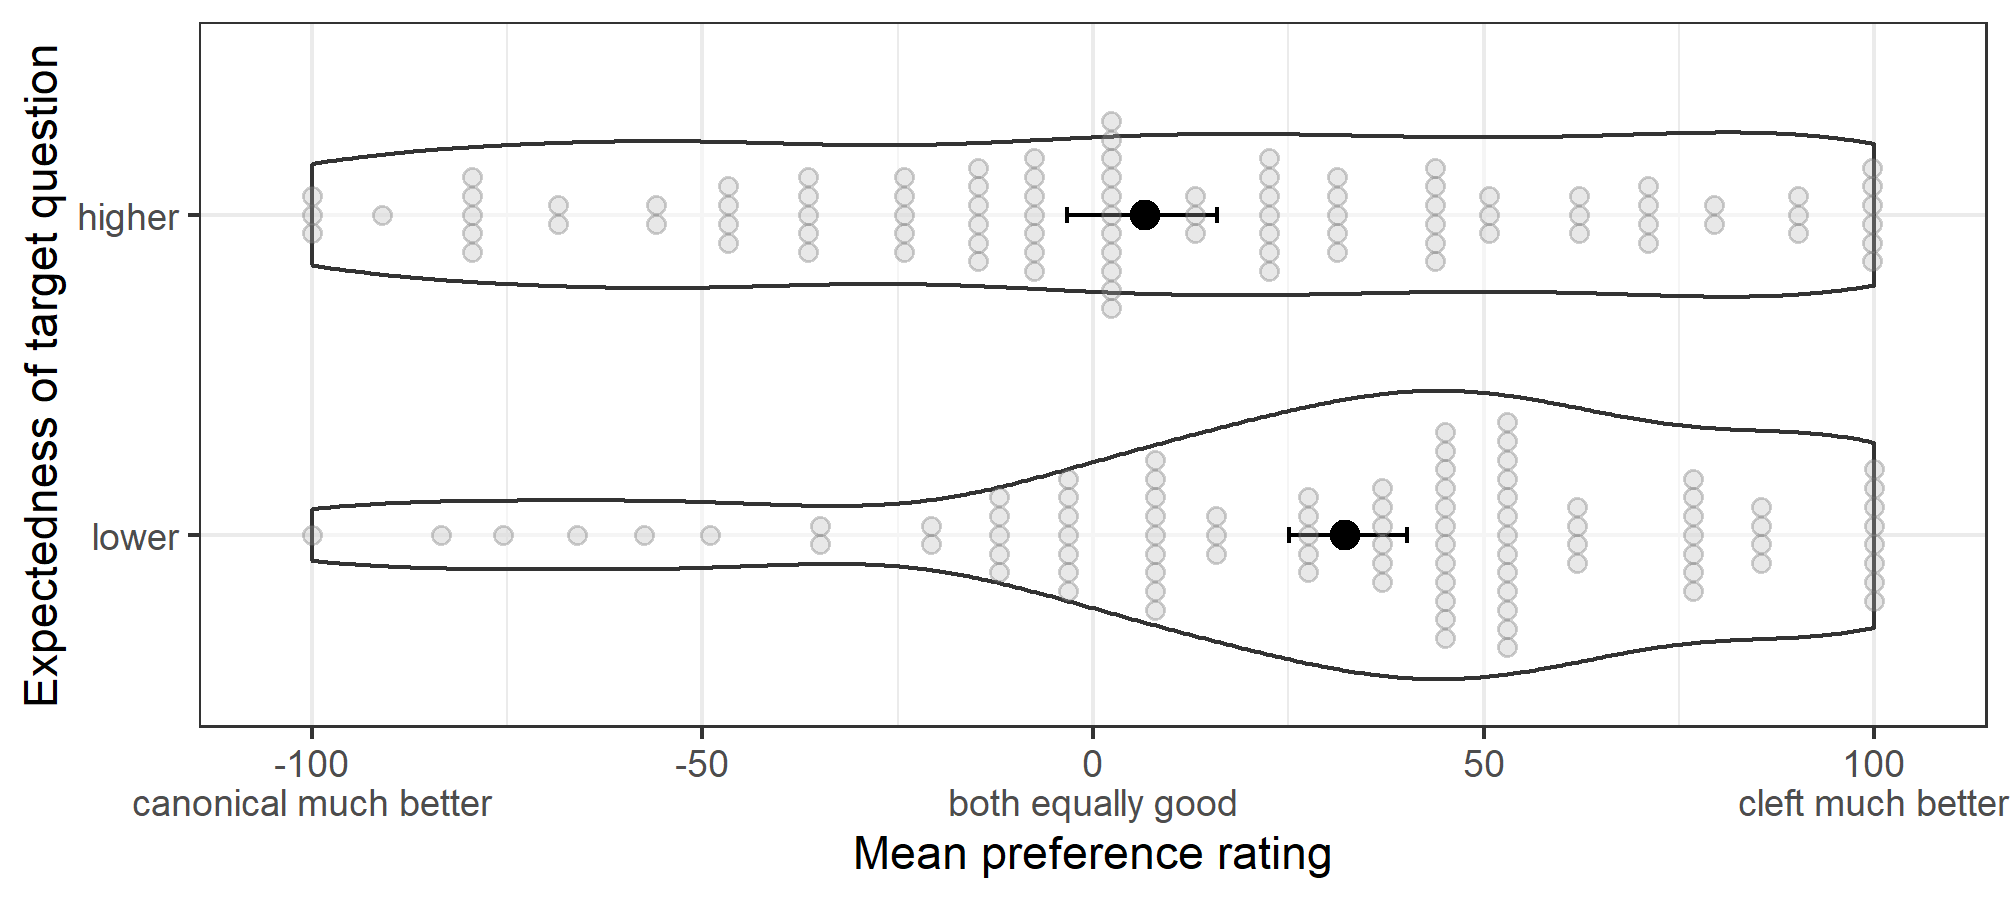
\includegraphics[width=1\textwidth]{results_main_experiment.png}
\end{center}
\label{fig:results_exp2}
\end{figure}


This result was confirmed by a linear mixed effects model that predicted the preference ratings from a fixed effect of context condition (reference level: higher expectedness) and random by-participant intercepts and slopes and by-item intercepts\footnote{Random by-item slopes were removed because there was a correlation of -1 with the fixed effect of context condition.} (R version 4.1.2, \textit{lme4} package). There was a main effect of context condition ($\beta=26$, \textit{SE} $=5.8$, $t=4.5$, $p<.001$), suggesting that participants' preference for the cleft over the canonical sentence was stronger when the target question was relatively less expected compared to when it was relatively more expected.


%============================ discussion ===========================
\section{Discussion}
\label{sec:discussion}

\subsection{Theoretical implications}

The experiment revealed that the context and the resulting expectations on how the text could develop significantly affect the relative acceptability of the German cleft compared to its canonical variant. The results confirm that there is a stronger preference for the cleft over the canonical sentence when the target question is relatively less expected than when it is relatively more expected. This partly supports  \citeauthor{tonnis_2021}' (\citeyear{tonnis_2021}) hypothesis, namely the part that German clefts address relatively unexpected questions. Since the two context conditions in the experiment did not differ with respect to exhaustivity, uniqueness, or contrast, theories of German clefts that primarily focus on such features cannot predict the attested differences. We argue that such theories need to be extended to account for the influence of discourse expectations on the acceptability of German clefts. \cite{tonnis_2021}, for instance, explained exhaustivity and contrast as side effects of the requirement for clefts to address a relatively unexpected question \cite[more details in][301--306]{tonnis_2021}.

However, in the context condition in which the target question was relatively more expected, such as \ref{context1}, the canonical sentence was not clearly preferred over the cleft. Hence, the part of the hypothesis that canonical sentences address relatively expected questions cannot be clearly confirmed.
 This may be due to the target question, which is relatively more expected in the higher expectedness condition compared to the lower expectedness condition, but might not be sufficiently expected in the higher expectedness condition to result in a preference of the canonical sentence over the cleft. This situation was anticipated in an additional hypothesis by \citet[256--261]{tonnis_2021}, which says that the cleft and the canonical sentence are equally acceptable when a question is addressed which is neither particularly expected nor particularly unexpected. The one sentence context \ref{context1} ({\em When Benni came into the shed, his bicycle was blocked}), could be such a case, if the target question \textit{Who parked in front of Benni's bicycle?}~is expected but not very strongly. The question \textit{How did he free his bicycle?}, for instance, might be relatively more expected in this context. We leave further exploration of the relative expectedness of questions to future research.

\subsection{Methodological implications}
\label{subsec:method_impl}

Our results imply that experiments designed to investigate factors that modulate the acceptability of German clefts should present the examples in a context to clarify the discourse expectations. If no such context is provided, participants' judgments might be influenced by the expectations created by the discourses that they imagine. 

The paradigm used in the norming study (henceforth referred to as the `question expectedness paradigm'; see Appendix A for a full description) allows researchers to measure the discourse expectations that clefts are sensitive to. The norming study confirmed \citeauthor{tonnis_2021}' (\citeyear[273ff.]{tonnis_2021}) assumption that a question that is raised by a sentence becomes less expected when the discourse proceeds. We expect this novel paradigm to be useful for measuring discourse expectations more generally. The question elicitation paradigms used in \cite{kehler_rohde_2017} and \cite{westera_rohde_2019}, for instance, ask participants to write down a question that comes to their mind after reading a context. Such paradigms, therefore, are very useful to identify the most expected questions in a context. These paradigms do not, however, allow the researcher to investigate questions that are salient but less expected. Thus, one advantage of the question expectedness paradigm is that it can be used to measure the expectedness of any question (independently of its expectedness), which makes it possible to study discourse expectations in more detail.  

A second advantage of the question expectedness paradigm over previously used paradigms is that it allows the researcher to measure the expectedness of a question in relation to other questions. This is useful, for instance, if one is interested in understanding how a change in the expectedness of one question affects the expectedness of another. For instance, the expectedness of the target question Q1 \textit{Who parked in front of Benni's bicycle?} in context \ref{context3} was measured in relation to four other questions. The questions Q2 \textit{What could Benni have used instead of the bicycle?} and Q3 \textit{Where did Benni go with the scooter?} were raised by the second and third sentence of the context, respectively. The other two questions were questions which we hypothesized to have a very high expectedness throughout the discourse (Q+ \textit{What did Benni do next?}), or a very low one (Q- \textit{How was the weather in Colombia?}). \autoref{fig:relative} plots the mean expectedness of these five questions by context condition. As predicted by \citeauthor{tonnis_2021}' (\citeyear[273ff.]{tonnis_2021}) hypothesis that newly raised questions can lower the expectedness of previously raised questions, the mean expectedness of the target question Q1 appeared to be higher than that of Q3 in the one sentence context condition, but the situation seems reversed in the three sentence context condition, where the third context sentence raises the expectedness of Q3. 

\begin{figure}[]
\caption{Mean expectedness rating with 95\% bootstrapped confidence intervals by context condition and question.}
\begin{center}
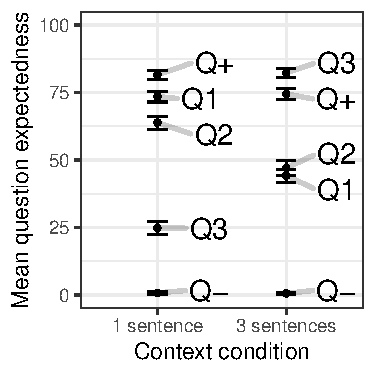
\includegraphics[width=.5\textwidth]{main_results_norming.pdf}
\end{center}
\label{fig:relative}
\end{figure}

The question expectedness paradigm can, we suggest, be fruitfully employed to empirically investigate a broad range of phenomena that have been analyzed as sensitive to questions and discourse expectations, such as indefinites \cite[e.g.,][]{onea_2016}, contrastive focus \cite[e.g.,][]{zimmermann_2011b}, at-issueness \cite[e.g.,][]{destruel_velleman_2014}, or projection inferences \cite[e.g.,][]{tbd-variability}.



\subsection{A closer look at the experiment stimuli}

As described in \autoref{subsec:material}, all the contexts used in this experiment were kept as similar as possible. We consider it necessary to control the contexts of the stimuli in such a strict way since small changes in the discourse structure might have a strong effect on the probability distribution over the questions the next sentence is likely to answer. Consider, for instance, the variant of the three sentence context in \ref{context3} given in \ref{context4}, where the third sentence does not move the story along, but instead continues to describe the same topic. In this context, we would expect the cleft and the canonical sentence to be rated as equally acceptable.
 \ex. Als Benni in den Schuppen kam, war sein Fahrrad zugestellt. Der Schuppen war sehr eng und vollgestopft. Jetzt stand auch noch ein pinkes Fahrrad vor seinem.\\
 \textit{`When Benni came into the shed his bicycle was blocked. The shed was very narrow and packed. On top of that, a pink bicycle now stood in front of his.'}\label{context4} 
 \a.\label{canonical4} Lilly hat vor Bennis Fahrrad geparkt.\\
\textit{`Lilly parked in front of Benni's bicycle.'}
\b.\label{cleft4}Es war Lilly, die vor Bennis Fahrrad geparkt hat.\\
\textit{`It was Lilly who parked in front of Benni's bicycle.'}

This example suggests that the critical property of the target stimuli in the experiment was not that the three sentence contexts consisted of three sentences but, rather, that the third sentence moved the story along. In other words, this example suggests that question expectedness may not be lowered purely by the number of intervening sentences but, rather, by the temporal properties of the story described. Future research should investigate more closely which linguistic and extralinguistic properties of discourses modulate question expectedness.

Finally, we consider the tense/aspect properties of the target sentences. The cleft sentences in the experiment consisted of a past tense main clause and a present perfect relative clause, while the canonical sentences realized a present perfect main clause. We used the present perfect in the canonical variants because it is the colloquial way of conveying past temporal reference in German \citep{van_der_klis_et_al_2017}. However, given that our stimuli were designed such that the third context sentence moved the discourse forward in time and the cleft/canonical continuation referred to the first sentence, it perhaps comes as no surprise that, in the three sentence discourse repeated in \ref{context6}, the past perfect canonical variant in \ref{canonical6} is relatively more acceptable than the present perfect canonical variant in \ref{canonical_perfekt6}.\vspace{-0.5ex}
 
 \ex.\label{context6} \textit{When Benni came into the shed his bicycle was blocked. He couldn't get it out quickly enough. So he set off on the scooter.}\label{context5}
 \a.\label{canonical6} Lilly \textbf{hatte} vor Bennis Fahrrad \textbf{geparkt}.\\
\textit{`Lilly \textbf{had parked} in front of Benni's bicycle.'}
 \b.?\label{canonical_perfekt6}Lilly hat vor Bennis Fahrrad geparkt.\\
\textit{`Lilly parked in front of Benni's bicycle.'}
\b.\label{cleft6}Es war Lilly, die vor Bennis Fahrrad geparkt hat.\\
\textit{`It was Lilly who parked in front of Benni's bicycle.'}

One might argue that the result of our experiment, that the cleft was preferred over the present perfect variant in the three sentence context, is not due to the target question being less expected, but because the present perfect is less suitable to express anteriority (see \cite{delin_oberlander_1992} for the claim that clefts can express anteriority). A piece of evidence speaking against this hypothesis is the observation that clefts are preferred over canonical present perfect variants even in contexts that do not require the expression of anteriority. In \ref{topic_shift}, for instance, the state of Anna being bored does not temporally follow the state of Lena flirting with some guy, namely Peter, but the cleft is nevertheless preferred over the present perfect canonical variant.  The past perfect variant in \ref{pastperfect}, which conventionally conveys anteriority, is less acceptable than the cleft in this context, as it suggests that Lena first flirted with some guy and then, later, with Peter (i.e., {\em Peter} is not coreferential with {\em some guy}), which leads to a less coherent continuation.\vspace{-0.5ex}
\ex.\label{topic_shift} Lena hat auf der Party mit einem Typen geflirtet. Sie hatte sehr viel Spaß. Anna war eher gelangweilt.\\
\textit{`Lena flirted with some guy at the party. She had a lot of fun. Anna was rather bored.'}
\a.\label{cleft5}Es war Peter, mit dem Lena geflirtet hat.\\
\textit{`It was Peter Lena flirted with.'}
\b.?\label{canonical5}Lena hat mit Peter geflirtet.\\
\textit{`Lena flirted with Peter.'}
\c.?\label{pastperfect}Lena hatte mit Peter geflirtet.\\ {\em `Lena had flirted with Peter.'}

Data like \ref{topic_shift} lead us to believe that considerations about which forms can express anteriority relations do not suffice to account for the target contrast we have investigated in this paper. Another hypothesis is that the past perfect may be another strategy to address relatively unexpected questions, given that it is, just as the cleft, a more marked form in German. Either way, interactions between sentence form and tense/aspect are worthy of future investigation.

%============================  Conclusions  =======================================
\section{Conclusions}
\label{sec:conclusions}

This paper provided empirical evidence for  \citeauthor{tonnis_2021}' (\citeyear{tonnis_2021}) hypothesis that German clefts are used to address relatively unexpected questions in discourse. Specifically, the experiment showed that clefts were judged to be more acceptable than their canonical variants in contexts in which they addressed a relatively less expected question. This result implies that analyses of German clefts cannot be limited to uniqueness, exhaustivity, or contrastivity, but should incorporate a sensitivity to question expectedness. 




%=====================================================================
\bibliography{mybib}

%=====================================================================
\newpage

\begin{addresses}
  \begin{address}
    \textbf{Swantje T\"onnis} \\
    Department of English Linguistics, University of Stuttgart\\
	Keplerstraße 17\\
	70174 Stuttgart, Germany\\
    \email{swantje.toennis@ling.uni-stuttgart.de}
  \end{address}\\
  \begin{address}
    \textbf{Judith Tonhauser }\\
    Department of English Linguistics, University of Stuttgart\\
    Keplerstraße 17\\
	70174 Stuttgart, Germany\\
    \email{judith.tonhauser@ling.uni-stuttgart.de}
  \end{address}
\end{addresses}

%=====================================================================

\appendix

\setcounter{table}{0}
\renewcommand{\thetable}{A\arabic{table}}

\setcounter{figure}{0}
\renewcommand{\thefigure}{A\arabic{figure}}

\newpage

\section{Norming study}\label{sec:appendix_b}

To ensure that the target questions of the main experiment were relatively less expected in the `lower expectedness' context than in the `higher expectedness' context, participants rated the expectedness of the target question as well as four other questions in the two contexts.

\subsection{Methods}

\paragraph{Participants.}

80 self-declared native speakers of German, recruited and paid (\pounds9.12 per hour) on \href{https://www.prolific.co/}{Prolific}, participated in the experiment (36 female, 44 male; ages 19--64 years, mean age 35). 

\paragraph{Materials.}

The stimuli consisted of the 32 contexts of the main experiment, that is, 16 contexts that only consisted of the target context sentence, as in \ref{context1}, and 16 contexts that consisted of the target context sentence followed by the additional sentences, as in \ref{context3}. For the full set of target stimuli see Supplement B of the Github repository mentioned in footnote \ref{github}.  

Each pair of contexts that shared the same target context sentence was paired with the same five questions: the target question and four other questions. \autoref{fig:stimulus_exp1} shows (the English translations of) the five questions for the context in \ref{context3}. The target question Q1, here {\em Who parked in front of Benni's bicycle?}, was hypothesized to be raised by the target context sentence. The questions Q2 \textit{What could Benni have used instead of the bicycle?} and Q3 \textit{Where did Benni go with the scooter?} were hypothesized to be raised by the second and third sentence of the context, respectively. (These sentences were absent when the context only consisted of the target context sentence.) We expected the target question to be relatively more expected immediately after the target context sentence (that is, in the one sentence context condition) than after the third sentence (that is, in the three sentence context condition). By contrast, we expected Q3 to be relatively less expected in the one sentence context condition than in the three sentence context condition. The other two questions served as control questions. We expected Q+ (here, \textit{What did Benni do next?}), which was always a question about what the character did next, to receive high expectedness ratings in both context conditions. In contrast, we expected Q- (here, \textit{How was the weather in Colombia?}), which was always an unrelated question, to receive low expectedness ratings in both context conditions.

The 32 contexts were distributed across two lists, so that each of the 16 target questions occurred only once per list and so that each list had eight stimuli in the one sentence context condition and eight in the three sentence context condition.  Each list also included the same 14 filler stimuli: these consisted of two one sentence, two three sentence, and 10 two sentence contexts followed by five questions each. The fillers were designed to distract from the structure of the target stimuli. Hence, they never used \textit{als} ‘when’, but either used no subjunction or a different one, like \textit{weil} `because' or \textit{bevor} `before'. The five questions of the filler stimuli were similar to the five questions of the target stimuli. They were designed to elicit ratings that range over the entire scale from `absolutely unexpected' to `very expected'. The filler stimuli of the norming study can be found in Supplement B of the GitHub repository mentioned in footnote \ref{github}.

\paragraph{Procedure.}

Participants were first introduced to the family of six, as in the main experiment. On each trial, they read a context (called `text') and were asked to rate, for each of the five questions, the likelihood that the next sentence of the text would be about that question. As shown in \autoref{fig:stimulus_exp1}, they gave their ratings on sliding scales labeled `(absolut unerwartbar)' (absolutely unexpected) on the left end (coded 0) and `(sehr erwartbar)' (very expected) on the right end (coded 100). Each question was formulated as an embedded question. Question order was randomized on each trial.

\begin{figure}[]
\caption{\small English translation of a sample trial of the question norming study (original in German). The sentences in brackets were only displayed in the three sentence condition. Question labels (target question Q1, Q2, Q3, Q-, Q+) were not presented to the participants.}
\footnotesize
Read the text in the box. What do you expect that the next sentence will be about? Rate the following proposals and adjust the slider accordingly.\vspace{1ex}

\begin{tcolorbox}
\textit{When Benni came into the shed his bicycle was blocked. (He couldn't get it out quickly enough. So he set off on the scooter.) ...}
\end{tcolorbox}

About who parked in front of Benni's bicycle.\hfill \textbf{[target question Q1]}\\

\includegraphics[width=0.8\textwidth]{slider.png}\vspace{-2ex}\\
\footnotesize(absolutely unexpected) \hspace{34ex} (very expected)\\
About what Benni could have used instead of the bicycle. \hfill [Q2]\\

\includegraphics[width=0.8\textwidth]{slider.png}\vspace{-2ex}\\
\footnotesize(absolutely unexpected) \hspace{34ex} (very expected)\\
About where Benni went with the scooter.\hfill [Q3]\\

\includegraphics[width=0.8\textwidth]{slider.png}\vspace{-2ex}\\
\footnotesize(absolutely unexpected) \hspace{34ex} (very expected)\\
About what Benni did next.\hfill [Q+]\\

\includegraphics[width=0.8\textwidth]{slider.png}\vspace{-2ex}\\
\footnotesize(absolutely unexpected) \hspace{34ex} (very expected)\\
About how the weather is in Colombia.\hfill [Q-]\\

\includegraphics[width=0.8\textwidth]{slider.png}\vspace{-2ex}\\
\footnotesize(absolutely unexpected) \hspace{34ex} (very expected)\\\normalsize
\label{fig:stimulus_exp1}
\end{figure}


\paragraph{Data exclusion.}

The data from two participants was excluded from the analysis because their mean expectedness ratings were more than two standard deviations higher than the group mean of Q- or more than two standard deviations lower than the group mean on Q+. Data from 78 participants entered the analysis (35 female, 43 male, age range 19--64 years, mean age 35).

\subsection{Results}

\autoref{fig:relative} plots the mean expectedness rating of the target question Q1, and the other questions, by context condition. As expected, the mean expectedness rating of the target question was higher immediately after the target context sentence (i.e., in the one sentence context condition) than when the target context sentence was followed by two additional sentences (i.e., in the three sentence context condition). This result was confirmed by a linear mixed effects model that predicted the expectedness ratings for the target question from context condition (reference level: one context sentence) and random by-participant and by-item intercepts and slopes.\footnote{An item consisted of a context, followed by the target question and four other questions.} There was a main effect of context condition 
 ($\beta=-29.3$, \textit{SE} $=2.2$, $t=-13.6$, $p<.001$), such that the target question was less expected in the three sentence context condition than in the one sentence context condition.
 
\end{document}
